\documentclass[14pt, a4paper]{article}
\usepackage[utf8]{inputenc}
\usepackage[russian]{babel}
\usepackage{multirow}
\usepackage{graphicx}

\title{\textbf{Отчет о выполнении лабораторной работы 1.3.1}}
\author{Калашников Михаил, Б03-205}
\date{}

\begin{document}

\maketitle

\centerline{\textbf{I. Определение модуля Юнга по измерениям растяжения проволоки}}

\begin{table}[!h]
\centering
\begin{tabular}{| c | c |}
\hline
Площадь поперечного & \\
сечения проволоки, $S$ & $0.42\ mm^2$ \\
Длина & \\
рычага, $r$ & $13\ mm$ \\
Длина & \\
проволоки, $l\pm\sigma_l$ & $175.5\pm 0.5\ cm$ \\
Расстояние от шкалы & \\
до зеркальца, $h\pm\sigma_h$ & $137.3\pm 0.5\ cm$ \\
\hline

\end{tabular}
\label{table1}
\caption{Параметры установки}
\end{table}

Формула, связывающая смещение изображения линейки $\Delta x$, величины $h$, $r$ и удлинение $\Delta l$:
\[\Delta x=\alpha h=\frac{\Delta l}{r}h\]
\[\Delta l=\Delta x\frac{r}{h}\]

Проведем измерения положения изображения линейки при постепенном увеличении и уменьшении нагрузки $\Delta m$ на проволоку. Рассчитаем смещение изображения относительно начального положения. Усредним полученные значения и вычислим среднекватратические отклонения по формуле:
\[\sigma_a=\sqrt{\frac{\sum_{i=1}^{N}\left(a-a_{i}\right)}{N\left(N-1\right)}}\]
\[\sigma_{\Delta x}=\sqrt{\frac{\sum_{i=1}^{N}\left(\Delta x-\Delta x_{i}\right)}{N\left(N-1\right)}}\]

После этого рассчитаем удлинение проволоки. Погрешность данной величины найдем по формуле:
\[\sigma_Y=\sqrt{\sum_{i=1}^N\left(\frac{\delta Y}{\delta X_i}\sigma_{X_i}\right)^2},\]
\[\sigma_{\Delta l}=\Delta l\sqrt{\left(\frac{\sigma_{\Delta x}}{\Delta x}\right)^{2}+\left(\frac{\sigma_{h}}{h}\right)^{2}}.\]

\newpage

\begin{table}[!h]
\centering
\begin{tabular}{| c | c | c | c | c | c |}

\hline
$\Delta m$, $g$ & 0.0 & 245.6 & 491.7 & 737.5 & 983.6 \\
\hline
\hline
\multirow{6}{*}{$x_i$, $cm$} 
& 17.6 & 18.9 & 20.0 & 20.9 & 22.0 \\
\cline{2-6}
& 17.3 & 18.6 & 19.9 & 21.1 & 22.0 \\
\cline{2-6}
& 17.3 & 18.8 & 19.8 & 21.0 & 22.1 \\
\cline{2-6}
& 17.4 & 18.5 & 19.8 & 20.9 & 22.1 \\
\cline{2-6}
& 17.3 & 18.5 & 19.6 & 20.9 & 22.0 \\
\cline{2-6}
& 17.2 & 18.5 & 19.5 & 20.7 & 22.0 \\
\hline
\hline
\multirow{6}{*}{$\Delta x_i$, $cm$}
& 0.0 & 1.3 & 2.4 & 3.3 & 4.4 \\
\cline{2-6}
& 0.0 & 1.3 & 2.6 & 3.8 & 4.7 \\
\cline{2-6}
& 0.0 & 1.5 & 2.5 & 3.7 & 4.8 \\
\cline{2-6}
& 0.0 & 1.1 & 2.4 & 3.5 & 4.7 \\
\cline{2-6}
& 0.0 & 1.2 & 2.3 & 3.6 & 4.7 \\
\cline{2-6}
& 0.0 & 1.3 & 2.3 & 3.5 & 4.8 \\
\hline
\hline
$\Delta x\pm\sigma_{\Delta x}$, $cm$ 
& 0.0 & $1.28\pm0.05$ & $2.42\pm0.05$ & $3.57\pm0.07$ & $4.68\pm0.06$ \\
\hline
$\Delta l\pm\sigma_{\Delta l}$, $mm$ 
& 0.0 & $0.12\pm0.005$ & $0.23\pm0.005$ & $0.34\pm0.007$ & $0.44\pm0.006$ \\
\hline

\end{tabular}
\label{table2}
\caption{Измерение положения изображения линейки и расчет удлинения проволоки}
\end{table}

Построим график зависимости $\Delta l(P)$, где $P=\Delta mg$ ($g=9.8154\ m\cdot s^{-2}$).

\begin{figure}[!h]
\centering
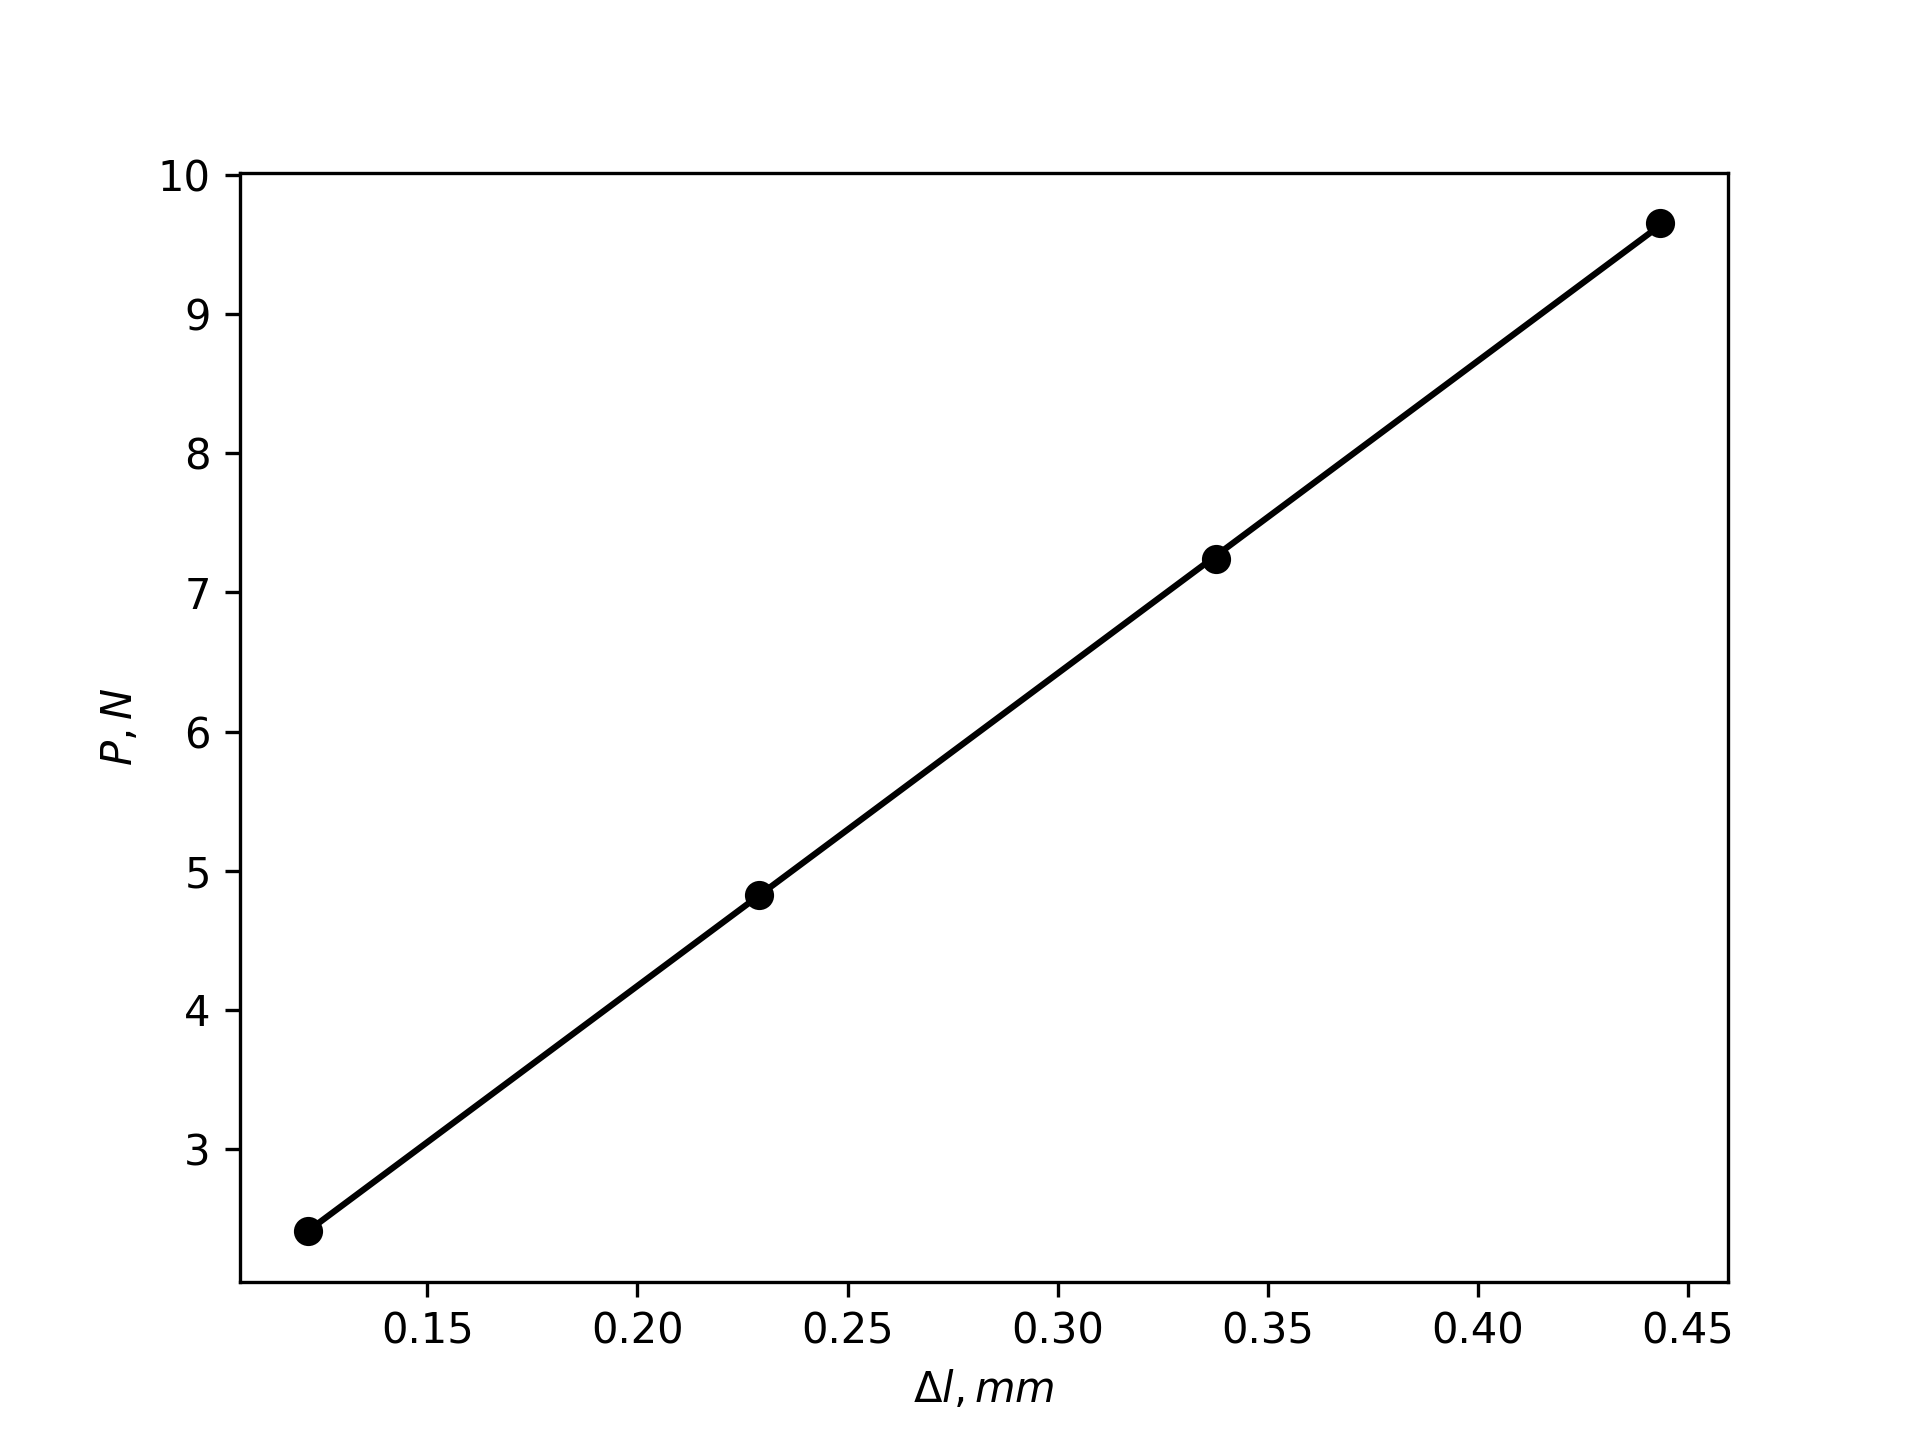
\includegraphics[scale=0.7]{laba6_1.png}
\label{image1}
\end{figure}

По графику определим, что $k=22.47\ kN\cdot m^{-1}$. Модуль Юнга найдем по формуле:
\[E=\frac{F}{S}\cdot\frac{l}{\Delta l}=k\frac{l}{S}=94.2\ GPa.\]
\[\sigma_E=E\frac{\sigma_l}{l}=k\frac{\sigma_l}{S}=0.3\ GPa\]

Данное значение соответсвует модулю Юнга латуни.

\newpage

\centerline{\textbf{II. Определение модуля Юнга по измерениям изгиба балки}}

Расстояние между призмами $l\pm\sigma_l=50\pm0.1\ cm$.

Эксперимент будет проводиться с тремя брусками: одним металлическим и двумя деревянными. Измерим их параметры.

\begin{table}[!h]
\centering
\begin{tabular}{| c | c | c | c | c | c | c | c | c | c | c |}

\hline
\multicolumn{11}{| c |}{Брусок №1 (металл)} \\
\hline
Толщина, $mm$ & 3.84 & 3.81 & 4.17 & 3.77 & 3.95 & 4.09 & 3.89 & 4.07 & 3.86 & 3.98 \\
\hline
Ширина, $mm$ & 21.21 & 21.30 & 21.21 & 21.27 & 21.10 & 21.13 & 21.30 & 21.47 & 21.28 & 21.21 \\
\hline
\multicolumn{11}{| c |}{Брусок №2 (дерево)} \\
\hline
Толщина, $mm$ & 10.45 & 10.39 & 10.05 & 10.06 & 10.24 & 10.48 & 10.55 & 10.32 & 10.32 & 10.40 \\
\hline
Ширина, $mm$ & 20.11 & 20.11 & 20.02 & 20.05 & 20.33 & 20.23 & 20.27 & 20.11 & 20.09 & 20.30 \\
\hline
\multicolumn{11}{| c |}{Брусок №3 (дерево)} \\
\hline
Толщина, $mm$ & 10.83 & 11.05 & 10.74 & 10.78 & 11.05 & 10.70 & 10.67 & 10.34 & 10.35 & 10.55 \\
\hline
Ширина, $mm$ & 18.89 & 18.57 & 18.52 & 18.55 & 18.77 & 18.80 & 19.31 & 19.26 & 18.93 & 18.64 \\
\hline

\end{tabular}
\label{table3}
\caption{Измерение геометрических параметров брусков}
\end{table}

\begin{table}[!h]
\centering
\begin{tabular}{| c | c | c | c |}

\hline
Брусок & 1 & 2 & 3 \\
\hline
Толщина, $b\pm\sigma_b$, $mm$ & $3.94\pm0.04$ & $10.33\pm0.05$ & $10.71\pm0.08$ \\
\hline
Ширина, $a\pm\sigma_a$, $mm$ & $21.25\pm0.03$ & $20.16\pm0.03$ & $	18.82\pm0.09$ \\
\hline

\end{tabular}
\label{table4}
\caption{Геометрические параметры брусков}
\end{table}

Проведем измерения относительного изменения значения прогиба при различной нагрузке и построим график зависимости $\Delta x(m)$.

\begin{table}[!h]
\centering
\begin{tabular}{| c | c | c | c | c | c | c | c | c |}

\hline
Брусок & Масса нагрузки, $m$, $g$ & 461.8 & 482.5 & 511.0 & 944.3 & 972.8 & 993.5 & 1455.3 \\
\hline
1 & \multirow{3}{*}{Смещение, $\Delta x$, $mm$}
& 0.67 & 0.70 & 0.72 & 1.28 & 1.31 & 1.33 & 1.96 \\
\cline{1-1}
\cline{3-9}
2 & & 0.58 & 0.63 & 0.62 & 1.15 & 1.19 & 1.23 & 1.74 \\
\cline{1-1}
\cline{3-9}
3 & & 0.4 & 0.45 & 0.47 & 0.79 & 0.88 & 0.84 & 1.22 \\
\hline

\end{tabular}
\label{table5}
\caption{Измерения величины деформации брусков}
\end{table}

Зная, что эти две велиничы связаны формулой
\[\Delta x=\frac{gl^{3}}{4ab^{3}E}m,\]
определим модуль Юнга из углового коэффициента $k$ прямой, проведенной через полученные точки:
\[E=\frac{gl^{3}}{4ab^{3}k},\]
\[\sigma_E=E\sqrt{\left(\frac{\sigma_a}{a}\right)^{2}+\left(3\frac{\sigma_b}{b}\right)^{2}+\left(3\frac{\sigma_l}{l}\right)^{2}}.\]

\newpage

\begin{figure}[!h]
\centering
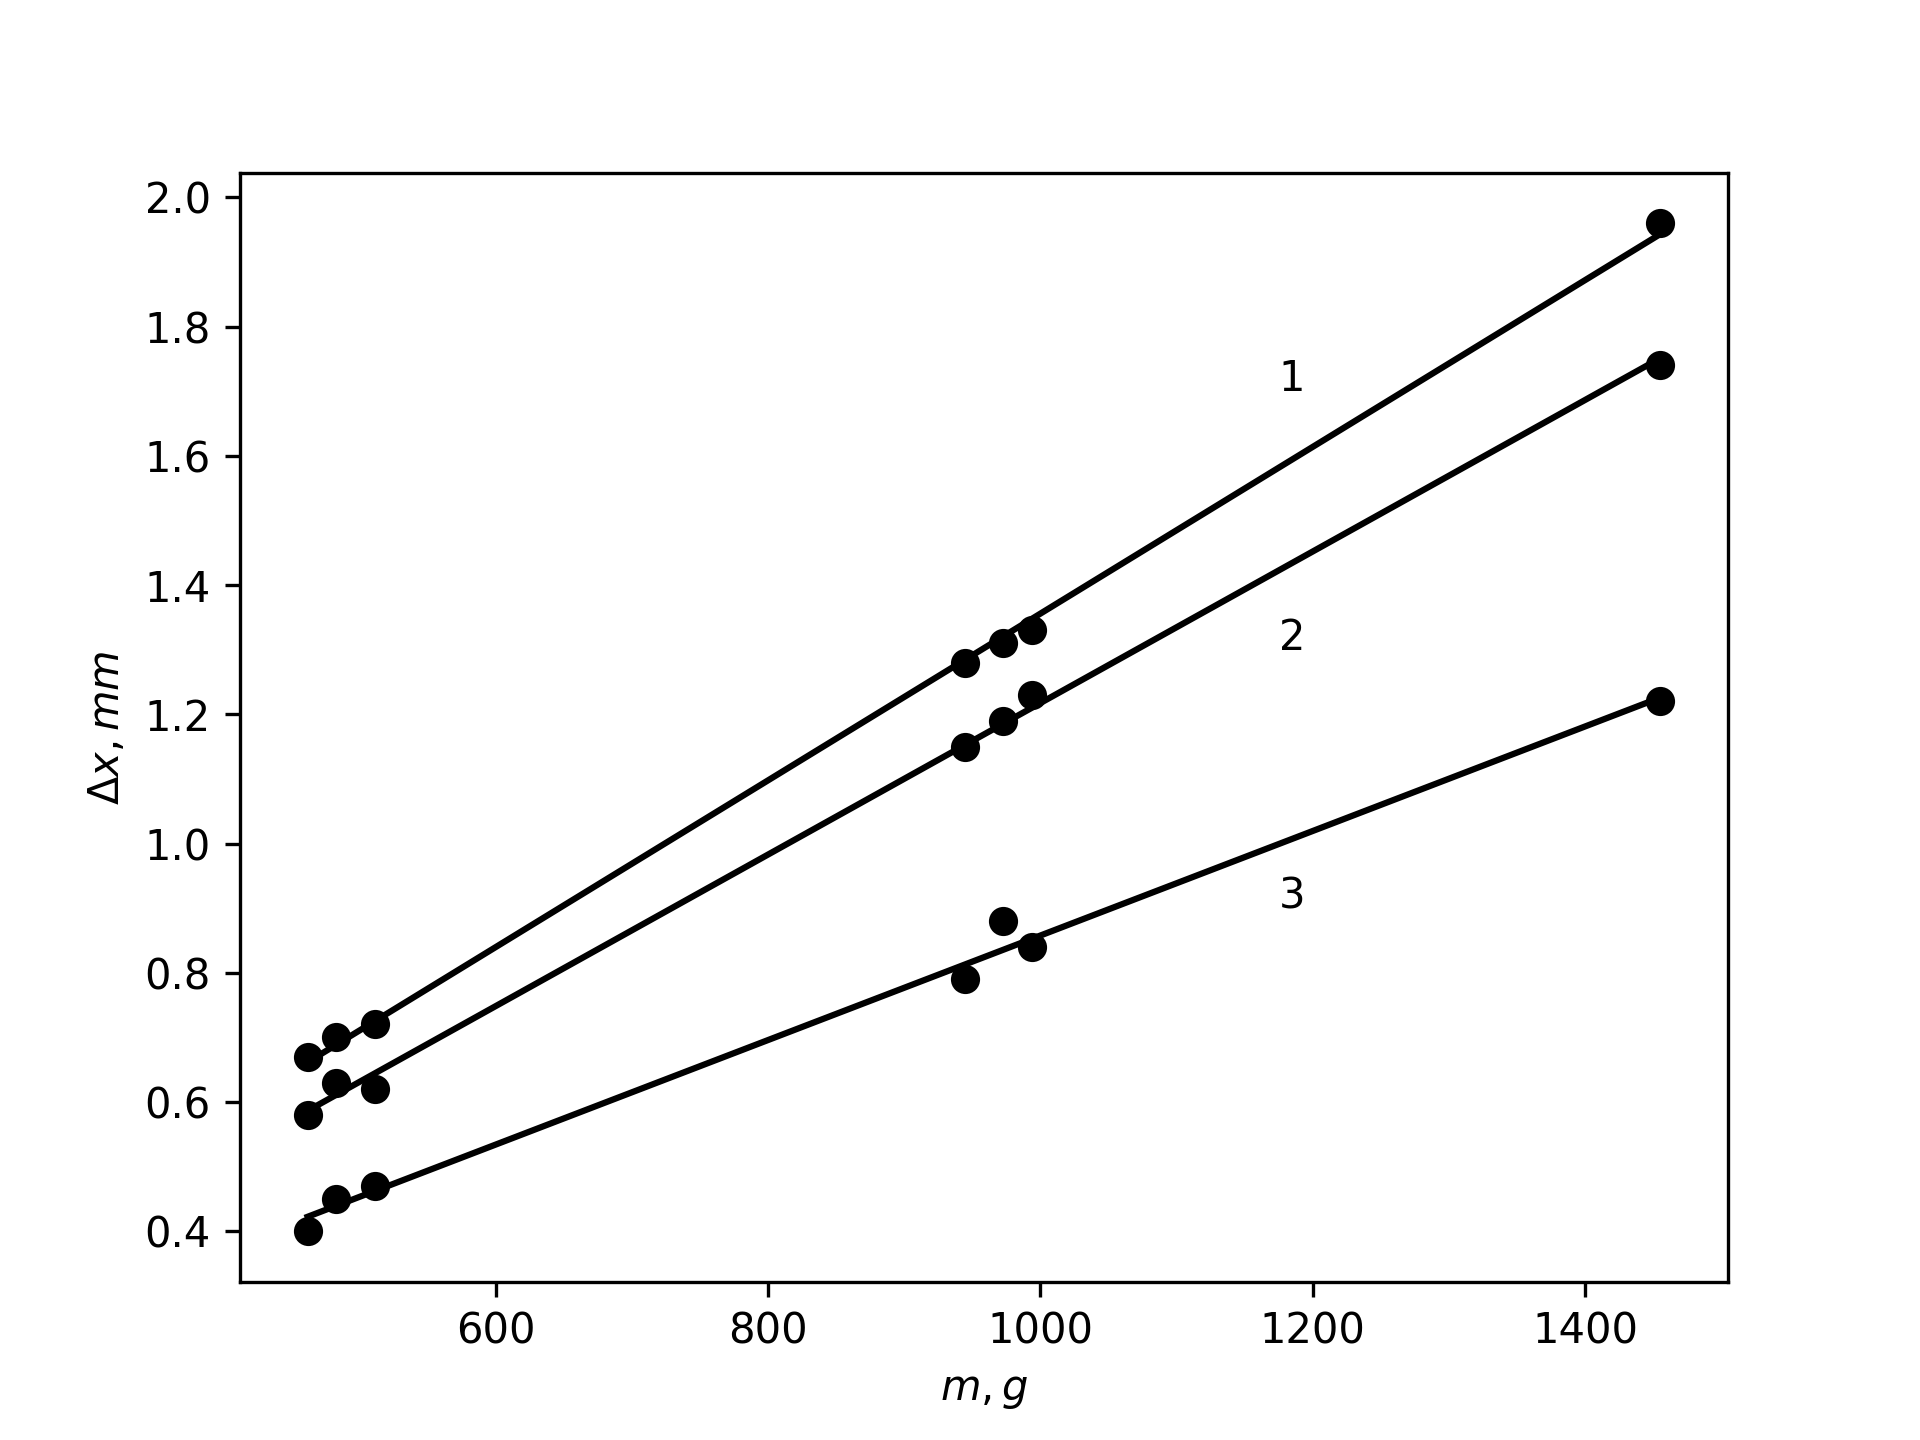
\includegraphics[scale=0.8]{laba6_2.png}
\label{image2}
\end{figure}

\begin{table}[!h]
\centering
\begin{tabular}{| c | c | c | c |}

\hline
Брусок & 1 & 2 & 3 \\
\hline
Коэффициент, $k$, $m\cdot g^{-1}$ & 1.29 & 1.17 & 0.81 \\
\hline
Модуль Юнга, $E$, $GPa$ & $182.5\pm 5.9$ & $11.8\pm0.2$ & $16.4\pm 0.4$ \\
\hline

\end{tabular}
\label{table6}
\caption{Модуль Юнга брусков}
\end{table}

\end{document}